\newpage
\section{Experiment 2: Acceptance of a Robot Programming Framework}

% \section{Can Users teach Action Models for Automated Planning using the Robot Programming Framework?}
\label{sec:Exp2}
%%%%%%%% 1.25 pages %%%%%%%

In this experiment, users were presented the robot programming framework (\chapt{chap:Contribution}), and had to teach action models by kinesthetic manipulation of a Baxter robot (Fig. \ref{fig:Baxter}). Users were instructed to demonstrate an atomic action and assign preconditions and effects. The goal was to assess the framework's usability and difficulties encountered, when teaching action models.

\subsection{Experimental Setup \& Participants}
We recruited 11 participants (7 male, 4 female), who were students and staff members at Universit\'{e} Grenoble Alpes. 6 participants reported programming experience with office productivity software (`beginner'), 2 had previously taken a programming course before (`advanced'), and 3 were pursuing studies in Computer Science (`expert').
%4 participants had previously heard of Automated Planning, but only 3 attended a related course.
The experiments were conducted using a Baxter robot (Fig. \ref{fig:Baxter}), mounted with a partial implementation of the framework (e.g. `learn a new action', `find an object', `execute an action sequence'). We used the Wizard-of-Oz technique to simulate the remaining functionalities (e.g. `generate action sequence').
Participants operated on a table with 2 positions (A and B), 2 cubes (blue and red), that represented parts on an assembly line. 
Each participant was allocated 1 hour, but the average duration was 29.5 minutes. The experiments were recorded, while the participant interacted with the robot. 


\begin{figure}[h]
	\centering
	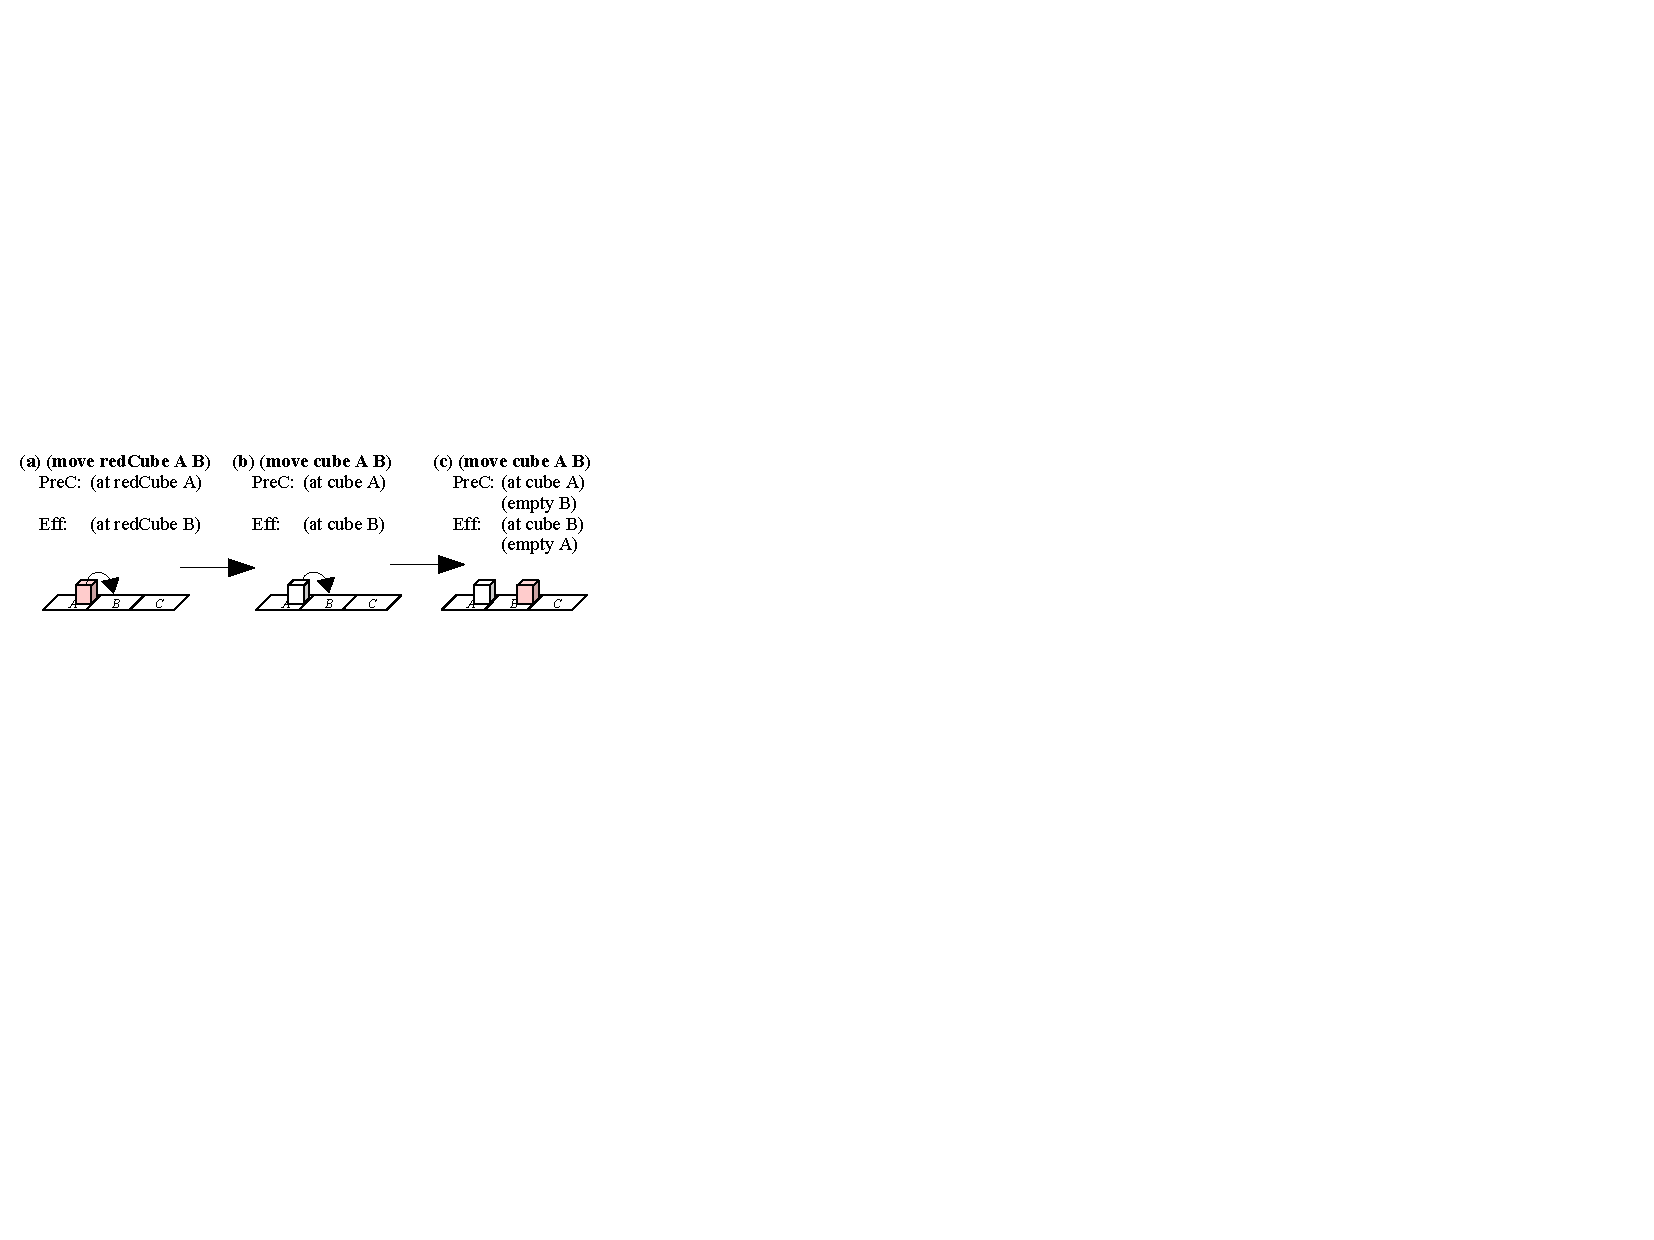
\includegraphics[width=0.8\linewidth]{figures/scenarios-exp2}
	\caption{Continuous refinement of the move action model: (a) initial action model learned by demonstration, (b) action model for all cubes of any colour, (c) action model with an additional condition, if the target position is occupied and cubes can not be stacked.}
	\label{fig:scenarios-exp2}
\end{figure} 
%The complete experimental protocol is shown in Fig. \ref{fig:Experimental protocol}. 
\subsection{Experimental Design \& Measurements}
The experiment was set in a simulated assembly line, where objects of the same shape, but different colour arrived consecutively at position A.
Users had to teach Baxter the action for moving an object from position A to position B, where objects should not be stacked. Throughout the experiment, users were faced with two different scenarios, where Baxter had to apply the learned action model. We evaluated the user's capability to refine action models, when faced with different situations, and wanted to assess the framework's overall usability.
The experiment consisted of the following phases:
\begin{itemize}
  %\item{Introduction: After a short introduction to the Baxter robot \cite{Baxter}, users were told that they needed to use a planning language (STRIPS) to explain Baxter the state of the world and the semantic meaning of the actions.}
  \item{\textbf{Training:} Users were shown how to manipulate Baxter's arm, and given time to familiarise themselves with the kinesthetic manipulation.}
  \item{\textbf{Experimental test:} Users were instructed to teach Baxter a move action of a cube. Then, they were presented the action model, with preconditions and effects, that Baxter learned from the demonstration (Fig. \ref{fig:scenarios-exp2}a). In the following, users were faced with two different scenarios, to refine the conditions of the action model. Starting with the initial action model for a red cube, users modified the conditions, so that it was applicable to all cubes of any colour (Fig. \ref{fig:scenarios-exp2}b), and when the target position was occupied (Fig. \ref{fig:scenarios-exp2}c). At each step, users observed how Baxter applied the learned action in the new scenario. When Baxter failed to execute the action, users had to refine the conditions of the action model.}
  \item{\textbf{Planning:} Users were presented a new scenario, where Baxter was instructed to achieve a new goal using the learned action model. The new goal was to switch the positions of two cubes on the table. Baxter demonstrated this by executing an action sequence generated by an automated planner.}
  \item{\textbf{Questionnaire:} Users were given a questionnaire containing 18 questions related to their experience (Fig. \ref{fig:eEvaluation}).}
   \item{ \textbf{Debriefing:} Users were questioned about their expectations on Baxter's behaviour, before applying the learned action model to a new scenario. Users were asked open-ended questions (``What will Baxter do when applying the learned action model?"), so that their responses were unbiased. When they encountered failure scenarios, they were asked to reason about Baxter's behaviour.} 
\end{itemize}

 \begin{figure}[ht]
  \centering
  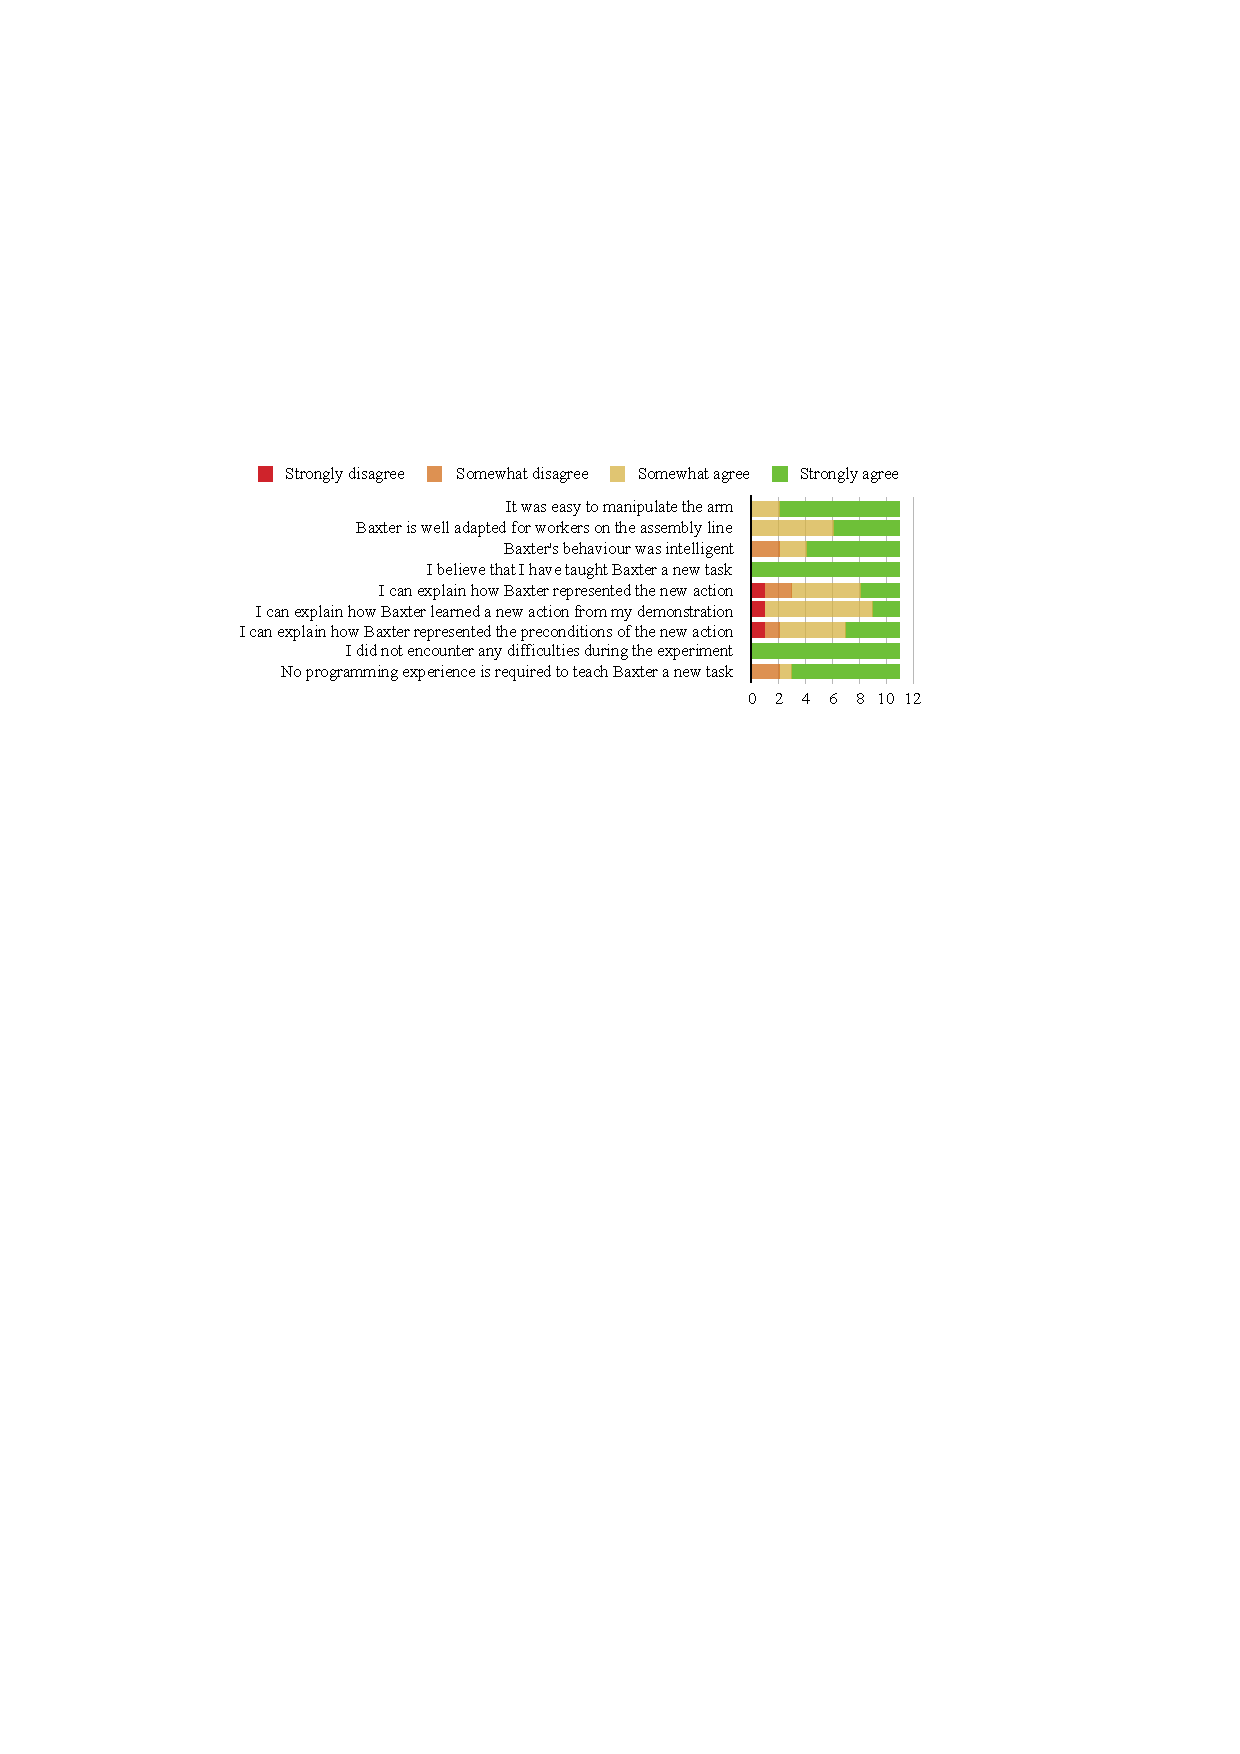
\includegraphics[width=\linewidth]{figures/eEvaluation}
  \caption{Summary of questionnaire responses: Extract of 18 questions on the user's understanding, after the experiment to teach action models by demonstration (Sec. \ref{sec:Exp2}).}
  \label{fig:eEvaluation}
\end{figure}


\subsection{Results}
%%%%%%%%%%%%%%%%%%%%%%%%%%%%%%%%%%%%%%%%%%%%%%%%%%%%%%%%%%%%%%%%%%%%%%%%%%%%%%%%
All (11) users were satisfied with the PbD process and Baxter's abilities to learn and reproduce the demonstrated move action. All users understood the learned action model and managed to adopt the notion of preconditions and effects easily. As expected, no users pointed out the missing conditions (Fig. \ref{fig:scenarios-exp2}c), when asked for improvements of the initial action model (Fig. \ref{fig:scenarios-exp2}a).
Even users who were `experts' and who had heard of automated planning before, did not manage to create a complete action model from the start. However, all users detected the missing condition easily, when faced with the relevant failure scenarios.

In the final phase, users with no experience in automated planning (8) did not expect Baxter to solve the permutation problem, and agreed unanimously that it acted in an intelligent manner, when it did. At the end of the experiment, all users believed that they had taught Baxter a new task and the majority understood the representation of the action models well. No users encountered any difficulties during the experiment. 8 participants believed that no programming experience was required to teach Baxter a task (Fig. \ref{fig:eEvaluation}).

